\documentclass[12pt,a4paper]{article}

% ============================================================
% PACKAGES
% ============================================================
\usepackage[a4paper,margin=1in]{geometry}
\usepackage{times}
\usepackage{setspace}
\usepackage{graphicx}
\usepackage{float}
\usepackage{booktabs}
\usepackage{array}
\usepackage{multirow}
\usepackage{longtable}
\usepackage{tabularx}
\usepackage{amsmath,amssymb}
\usepackage{algorithm}
\usepackage{algpseudocode}
\usepackage{xcolor}
\usepackage{listings}
\usepackage{tikz}
\usepackage{pgfplots}
\usepackage{caption}
\usepackage{subcaption}
\usepackage{hyperref}
\usepackage{enumitem}
\usepackage{fancyhdr}
\usepackage{titlesec}

\usetikzlibrary{
    shapes.geometric,
    arrows.meta,
    positioning,
    fit,
    calc
}

\pgfplotsset{compat=1.18}

% ============================================================
% HYPERLINKS
% ============================================================
\hypersetup{
    colorlinks=true,
    linkcolor=blue,
    citecolor=blue,
    urlcolor=blue,
    pdftitle={Compiler Design and Its Applications in ML, UML and Web Programming}
}

% ============================================================
% LINE SPACING
% ============================================================
\onehalfspacing

% ============================================================
% HEADER / FOOTER
% ============================================================
\pagestyle{fancy}
\fancyhf{}
\fancyhead[L]{Compiler Design Lab -- CSE3024}
\fancyhead[R]{VIT-AP University}
\fancyfoot[C]{\thepage}

% ============================================================
% CODE STYLE
% ============================================================
\definecolor{codegreen}{rgb}{0,0.5,0}
\definecolor{codegray}{rgb}{0.5,0.5,0.5}
\definecolor{codepurple}{rgb}{0.58,0,0.82}

\lstset{
    language=C,
    basicstyle=\ttfamily\small,
    keywordstyle=\color{blue},
    commentstyle=\color{codegreen},
    stringstyle=\color{codepurple},
    numbers=left,
    numberstyle=\tiny\color{codegray},
    stepnumber=1,
    numbersep=8pt,
    frame=single,
    breaklines=true,
    showstringspaces=false
}

% ============================================================
% TITLE FORMAT
% ============================================================
\titleformat{\section}
{\large\bfseries}
{\thesection.}{0.5em}{}

\titleformat{\subsection}
{\normalsize\bfseries}
{\thesubsection}{0.5em}{}

% ============================================================
% DOCUMENT
% ============================================================
% ============================================================
% HELPER: red placeholders you must replace with your own words
% ============================================================
\newcommand{\todo}[1]{\textcolor{red}{\textit{[#1]}}}

\begin{document}

% ============================================================
% TITLE PAGE
% ============================================================
\begin{titlepage}
\begin{center}

\vspace*{0.5cm}
{\Large\bfseries VIT-AP UNIVERSITY}
\vspace{0.3cm}

{\large Amaravati, Andhra Pradesh, India}
\vspace{1.2cm}

{\Large\bfseries COMPILER DESIGN LAB REPORT}
\vspace{0.4cm}

{\large \textbf{Subject Name: Compiler Design Lab}}
\vspace{0.15cm}

{\large \textbf{Course Code: CSE3024}}
\vspace{1cm}

{\LARGE\bfseries
ML-Driven Intermediate Code Optimization:\\
A Framework for Automatic Code Improvement
}
\vspace{1.2cm}

\textbf{Submitted by}
\vspace{0.4cm}

\begin{tabular}{ll}
\textbf{Student 1 Name} & \textbf{Regd. No.:} XXXXXXXX \\[0.4cm]
\textbf{Student 2 Name} & \textbf{Regd. No.:} XXXXXXXX \\
\end{tabular}
\vspace{1.2cm}

\textbf{Under the Guidance of}
\vspace{0.3cm}

\textbf{Dr. Prakash Kumar Sarangi}
\vspace{1cm}

{\large
School of Computer Science and Engineering (SCOPE)\\
VIT-AP University\\
Amaravati, Andhra Pradesh, India
}
\vspace{0.4cm}

{\large Academic Year 2026--2027}

\end{center}
\end{titlepage}

% ============================================================
% ABSTRACT
% ============================================================
\section*{Abstract}

Compilers improve intermediate code by applying optimization techniques such as constant folding, strength reduction, common subexpression elimination, copy propagation and dead-code elimination. Production compilers usually apply these techniques in a fixed order to every program, which wastes compile effort on techniques that give no benefit to a particular program. This report presents a machine learning framework that predicts which sequence of optimization techniques should be applied to a three-address code program. Each program is described by 22 static features, and a classifier chooses one of ten candidate technique sequences. A dataset of 6{,}000 generated programs was labelled by applying every sequence and measuring the resulting cost, and four classifiers were compared with a fixed full sequence, hand-written rules and an oracle. Logistic Regression performed best: it reduced program cost by 69.6\% compared with 70.9\% for the fixed sequence, while running 5.1 techniques per program instead of 9. A confidence-threshold extension allows the framework to trade compile effort against code quality. The programs are synthetic and straight-line, so the results should be confirmed on real code.

\vspace{0.3cm}
\textbf{Keywords:}
Compiler Design, Intermediate Code, Three-Address Code, Code Optimization,
Phase Ordering, Machine Learning.

\newpage

% ============================================================
% INTRODUCTION
% ============================================================
\section{Introduction}

A compiler translates a program written in a source language into an equivalent program in a target language. In most compilers the source program is first converted into an intermediate representation (IR) such as three-address code, in which every instruction has at most one operator. The IR is then improved by the optimization phase and finally translated into machine code \cite{aho2006,cooper2007}. Working on an IR is convenient because the optimizations become independent of both the source language and the target machine.

Optimization aims to make a program cheaper, for example by using fewer or less expensive instructions, without changing what the program computes. Classical techniques include constant folding, algebraic simplification and strength reduction, common subexpression elimination, copy propagation and dead-code elimination \cite{muchnick1997}. This work implements these five techniques on three-address code.

Production compilers such as GCC and LLVM group techniques into fixed optimization levels and run them in a predetermined order. Programs, however, are different: a program with no repeated expressions gains nothing from common subexpression elimination, and one technique can create work for another. For example, copy propagation often produces dead code that is then removed by dead-code elimination. Choosing which techniques to run, and in which order, is known as the phase-ordering problem, and it has been studied with machine learning in compiler research \cite{cummins2021,liang2023}.

In this report, a classifier predicts a sequence of optimization techniques for each program from simple static features of its three-address code. The selected techniques are applied and the result is checked against the original program. The rest of the report is organised as follows: Section 2 reviews related work, Section 3 describes the methodology, Section 4 presents the results, and Section 5 concludes the report.

\subsection{Motivation}

A fixed technique order treats every program in the same way. Running every technique on every program is safe, but it spends compile time on techniques that have nothing to improve. If a model can recognise from cheap static features which techniques are useful, the compiler can skip the rest and compile faster. A small and transparent framework is also useful for understanding how optimization techniques interact, which is a core topic in compiler design.

\subsection{Problem Statement}

\textbf{Input:} an unoptimized three-address code (TAC) program.
\textbf{Output:} an optimized TAC program that computes the same results at lower cost.
The problem addressed is:

\begin{quote}
\textit{Given a TAC program, which sequence of optimization techniques should
be applied so that the program cost is close to the best achievable cost while
running as few techniques as possible?}
\end{quote}

The difficulty is that the number of possible technique orders grows quickly with the number of techniques, and trying every order on every program would cost more than it saves. A cheap way of choosing a good sequence for each program is therefore needed.

\subsection{Objectives}

\begin{enumerate}
    \item To implement a three-address-code intermediate representation with a
    cost model and five optimization techniques.
    \item To generate a labelled dataset by measuring the cost of every
    candidate technique sequence on every program.
    \item To train machine learning classifiers that predict the best technique
    sequence from static program features.
    \item To compare the classifiers against a fixed full sequence,
    hand-written rules and an oracle, and to evaluate a confidence-threshold
    extension.
\end{enumerate}

\subsection{Contributions}

\begin{itemize}
    \item \textbf{Optimization framework:} a TAC front end and five verified
    optimization techniques (constant folding, algebraic simplification and
    strength reduction, common subexpression elimination, copy propagation,
    dead-code elimination).
    \item \textbf{Dataset and labelling:} 6{,}000 de-duplicated programs, each
    labelled with its measured best technique sequence.
    \item \textbf{Learned selection:} a comparison of four classifiers with
    baselines, showing a reduction in compile effort with a small loss in code
    quality.
    \item \textbf{Confidence fallback:} an extension that applies the full
    sequence when the model is unsure, giving a tunable effort--quality
    trade-off.
\end{itemize}

\newpage

% ============================================================
% RELATED WORK
% ============================================================
\section{Related Work}


\subsection{Classical Compiler Optimization}

Aho et al. describe the standard compiler phases and the classical machine-independent optimizations \cite{aho2006}. Cooper and Torczon discuss how these optimizations are implemented in practice and how they interact \cite{cooper2007}, and Muchnick gives a detailed treatment of optimization algorithms \cite{muchnick1997}. The five techniques used in this work come from this classical body of work, where the techniques are applied by the compiler designer in a fixed order.

\subsection{Machine Learning for Phase Ordering}

Several researchers have applied machine learning to the choice and ordering of compiler optimizations. CompilerGym provides a Python environment in which LLVM phase ordering can be treated as a learning problem, together with benchmark datasets \cite{cummins2021}. Liang et al. learn a policy that selects optimization pass orders from a small set of good sequences and report an improvement over the default -Oz setting on unseen programs \cite{liang2023}. Our design is related to this idea because we also select from a small fixed set of sequences. The difference is scale and purpose: we work on a simple three-address IR with five transparent techniques, so that every step can be inspected and explained.

\subsection{Survey of Related Approaches}

\begin{table}[H]
\centering
\caption{Comparison of related approaches and the proposed framework}
\label{tab:survey}
\small
\begin{tabularx}{\textwidth}{p{2.6cm}p{2.6cm}X p{2.6cm}}
\toprule
\textbf{Approach} & \textbf{IR / Platform} & \textbf{Major Contribution} &
\textbf{Limitation}\\
\midrule
Fixed pipeline (e.g.\ -O2) & LLVM / GCC & Same technique order for all programs & Wastes effort on unhelpful techniques\\
Liang et al. \cite{liang2023} & LLVM IR & Learns to select pass sequences from a small set of good sequences & Needs LLVM tooling\\
CompilerGym \cite{cummins2021} & LLVM IR & Python environment for studying LLVM optimization with learning & Needs LLVM tooling; internals harder to inspect\\
\textbf{This work} & Three-address code & Transparent, small-scale framework; verified techniques; rule-based baseline; confidence fallback & Synthetic straight-line programs; simplified cost model\\
\bottomrule
\end{tabularx}
\end{table}

\subsection{Research Gap}

Existing machine learning approaches work on real LLVM IR and need large infrastructure, which makes them harder to reproduce and inspect at small scale. To our knowledge, there is limited transparent work that compares a learned technique selector with a fixed pipeline and with hand-written rules on a simple IR while also verifying correctness. This report addresses that gap with a lightweight framework. The general idea of learning optimization order is not new; the contribution here is the small and reproducible framework, the comparison, and the confidence-fallback extension.

\newpage

% ============================================================
% PROPOSED METHODOLOGY
% ============================================================
\section{Proposed Methodology}

\subsection{Proposed Workflow}

\begin{enumerate}
    \item Generate or accept a TAC program.
    \item Extract 22 static features from the unoptimized program.
    \item Predict the technique sequence with the trained classifier.
    \item If the prediction confidence is low, use the full sequence instead.
    \item Apply the chosen techniques to obtain the optimized TAC.
    \item Verify that the optimized program gives the same outputs, and report
    the cost reduction.
\end{enumerate}

\subsection{Proposed Flow Diagram}

\begin{figure}[H]
\centering
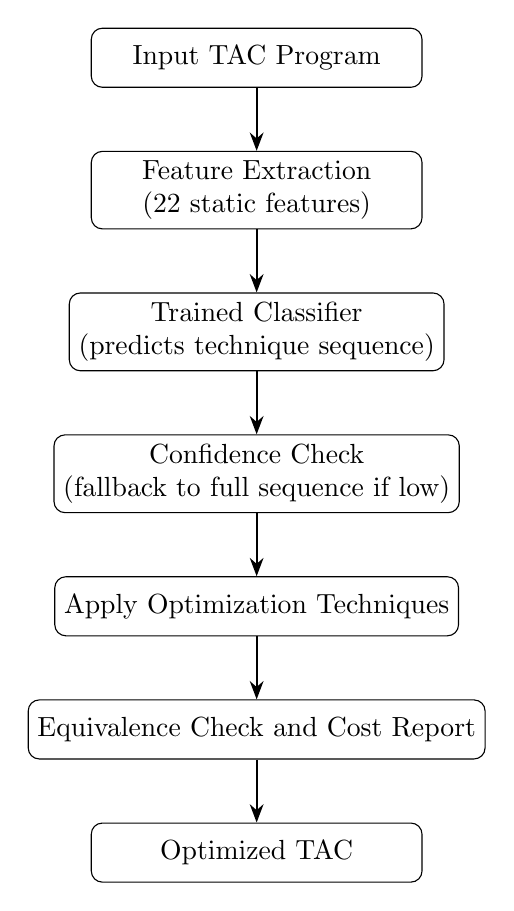
\begin{tikzpicture}[
node distance=0.8cm,
box/.style={rectangle,rounded corners,draw,minimum width=4.2cm,minimum height=0.75cm,align=center},
arrow/.style={-{Stealth},thick}
]
\node[box] (input) {Input TAC Program};
\node[box,below=of input] (feat) {Feature Extraction\\(22 static features)};
\node[box,below=of feat] (ml) {Trained Classifier\\(predicts technique sequence)};
\node[box,below=of ml] (conf) {Confidence Check\\(fallback to full sequence if low)};
\node[box,below=of conf] (apply) {Apply Optimization Techniques};
\node[box,below=of apply] (ver) {Equivalence Check and Cost Report};
\node[box,below=of ver] (out) {Optimized TAC};
\draw[arrow] (input) -- (feat);
\draw[arrow] (feat) -- (ml);
\draw[arrow] (ml) -- (conf);
\draw[arrow] (conf) -- (apply);
\draw[arrow] (apply) -- (ver);
\draw[arrow] (ver) -- (out);
\end{tikzpicture}
\caption{Proposed ML-driven optimization framework.}
\label{fig:workflow}
\end{figure}

\subsection{Intermediate Representation and Cost Model}

Each instruction is a tuple $(dst, op, a, b)$ with
$op \in \{copy, +, -, \times, \div, \ll, \gg\}$. A program has input variables
and output variables. For example, $x = a + b \times c$ becomes:

\begin{align}
t_1 &= b \times c\\
t_2 &= a + t_1\\
x &= t_2
\end{align}

The cost of a program is the sum of the instruction costs:
\begin{equation}
C(P) = \sum_{i \in P} c(op_i)
\end{equation}
where $c = 1$ for copy, add, subtract and shifts, $c = 3$ for multiply and
$c = 8$ for integer divide. This is a simplified latency-style model, not a
measurement on real hardware.

\subsection{Optimization Techniques}

\begin{table}[H]
\centering
\caption{Implemented optimization techniques}
\label{tab:techniques}
\small
\begin{tabularx}{\textwidth}{p{3.8cm}Xp{4.2cm}}
\toprule
\textbf{Technique} & \textbf{Idea} & \textbf{Example}\\
\midrule
Constant folding (with propagation) & Evaluate constant expressions at compile time & $3 \times 4 \rightarrow 12$\\
Algebraic simplification and strength reduction & Remove identities; replace costly operations by cheaper ones & $a \times 1 \rightarrow a$; $a \times 8 \rightarrow a \ll 3$\\
Common subexpression elimination & Reuse an already computed value & second $a+b$ becomes a copy\\
Copy propagation & Replace a copied variable by its source & $y=x;\ z=y+1 \rightarrow z=x+1$\\
Dead-code elimination & Delete instructions whose result is never used & unused $t_5 = a \times b$ removed\\
\bottomrule
\end{tabularx}
\end{table}

\subsection{Candidate Technique Sequences}

The classifier chooses one of ten candidate sequences. S9 (the full sequence
run twice) serves as the fixed baseline, similar in spirit to a fixed -O2-style
pipeline.

\begin{table}[H]
\centering
\caption{Candidate technique sequences (the ten classes)}
\label{tab:sequences}
\small
\begin{tabularx}{\textwidth}{p{2.6cm}X r}
\toprule
\textbf{Class} & \textbf{Techniques applied in order} & \textbf{Programs}\\
\midrule
S0\_none & (none) & 13\\
S1\_dce & DCE & 64\\
S2\_cf & CF, DCE & 539\\
S3\_alg & ALG, DCE & 353\\
S4\_cse & CSE, CP, DCE & 234\\
S5\_cf\_alg & CF, ALG, DCE & 674\\
S6\_cf\_cse & CF, CSE, CP, DCE & 218\\
S7\_alg\_cse & ALG, CSE, CP, DCE & 1394\\
S8\_full & CF, ALG, CSE, CP, DCE & 978\\
S9\_full\_x2 & CF, ALG, CSE, CP, DCE, CF, ALG, CP, DCE & 1533\\
\bottomrule
\end{tabularx}
\end{table}
\noindent CF = constant folding, ALG = algebraic simplification/strength
reduction, CSE = common subexpression elimination, CP = copy propagation,
DCE = dead-code elimination.

\subsection{Labelling}

For every program, all ten sequences are applied and the cost after each is
computed. The label is the sequence with the lowest cost; if several tie, the
one with the fewest techniques is chosen. Labels are therefore measured, not
estimated.

\subsection{Feature Extraction}

Each program is described by 22 numbers computed from the unoptimized TAC:
number of instructions; counts of add, subtract, multiply, divide and copy
instructions; constant-only operations; operations with a constant operand;
repeated expressions; identity operations; multiplications and divisions by
powers of two; dead instructions; reassigned variables; number of outputs;
number of unique variables; and the fractions of constant, duplicate, dead,
power-of-two, copy and identity instructions.

\subsection{Machine Learning Models}

Four classifiers are compared: Logistic Regression (with standardization),
Decision Tree (maximum depth 10), Random Forest (300 trees) and Gradient
Boosting (200 iterations). Logistic Regression is a simple linear baseline, the Decision Tree is easy to interpret, and Random Forest and Gradient Boosting are tree ensembles that handle count features and non-linear interactions well on tabular data.

\subsection{Baselines}

(a) No optimization; (b) fixed full sequence S9; (c) majority-class predictor;
(d) hand-written rules (apply constant folding if constant-only operations
exist, algebraic simplification if identities or powers of two exist, common
subexpression elimination if repeated expressions exist); (e) oracle, the true
best sequence, used as an upper bound.

\subsection{Proposed Extension: Confidence Fallback}

If the highest predicted class probability is below a threshold $\tau$, the
framework applies the full sequence S9 instead of the predicted one. Increasing
$\tau$ moves the policy from the learned selector towards the fixed pipeline.

\subsection{Proposed Algorithm}

\begin{algorithm}[H]
\caption{ML-Driven Technique Selection and Optimization}
\label{alg:main}
\begin{algorithmic}[1]
\Require TAC program $P$, trained classifier $M$, threshold $\tau$
\Ensure Optimized program $P'$
\State $f \gets$ ExtractFeatures($P$)
\State $p \gets M.\text{predict\_proba}(f)$
\State $s \gets \arg\max p$
\If{$\max p < \tau$}
    \State $s \gets$ S9 (full sequence)
\EndIf
\State $P' \gets P$
\For{each technique $t$ in sequence $s$}
    \State $P' \gets t(P')$
\EndFor
\State Verify $P'$ is equivalent to $P$ on random inputs
\State \Return $P'$
\end{algorithmic}
\end{algorithm}

\newpage

% ============================================================
% RESULTS
% ============================================================
\section{Results and Discussion}

\subsection{Dataset Preparation}

No public dataset was used. Programs were produced by the authors' generator;
each program receives a random profile (probabilities of constants, repeated
expressions, powers of two, identities, copies, dead statements and
reassignments) so that different techniques win on different programs. The
dataset has 6{,}000 unique programs with 23.8 instructions on average; exact
duplicates were removed. It was split 80\%/20\% (stratified, seed 42) into
training and test sets, and five-fold cross-validation was used on the training
set. The code asserts that no identical program appears in both sets. Features
are computed only from the unoptimized program.

\begin{table}[H]
\centering
\caption{Dataset summary}
\label{tab:dataset}
\begin{tabular}{lr}
\toprule
\textbf{Item} & \textbf{Value}\\
\midrule
Total programs & 6{,}000\\
Training programs & 4{,}800\\
Test programs & 1{,}200\\
Mean instructions per program & 23.8\\
Features per program & 22\\
Classes (technique sequences) & 10\\
Robustness set (45--90 instructions) & 1{,}200\\
\bottomrule
\end{tabular}
\end{table}

\begin{figure}[H]
\centering
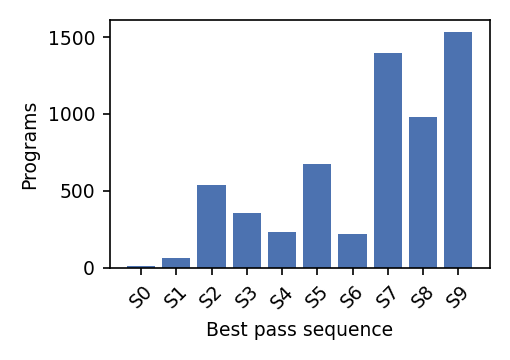
\includegraphics[width=0.55\textwidth]{fig_label_dist.png}
\caption{Distribution of best technique sequences in the dataset.}
\label{fig:labels}
\end{figure}

\subsection{System Requirements}

\begin{table}[H]
\centering
\caption{System requirements}
\begin{tabular}{ll}
\toprule
\textbf{Component} & \textbf{Requirement}\\
\midrule
Programming language & Python 3.12\\
Libraries & NumPy, scikit-learn 1.8.0, matplotlib, pandas\\
Hardware used & \todo{write your own computer or Colab details}\\
Run time of full experiment & about 50 seconds\\
\bottomrule
\end{tabular}
\end{table}

\subsection{Evaluation Metrics}

Classification quality is measured with accuracy and macro-averaged precision,
recall and F1-score over the ten classes. Because many sequences tie in cost,
three task-specific measures are also reported.

\begin{equation}
\text{Cost reduction} = \frac{\sum C(P) - \sum C(P')}{\sum C(P)} \times 100
\end{equation}

\begin{equation}
\text{Cost-optimal rate} = \frac{1}{N}\sum_{i=1}^{N}
\mathbb{1}\left[C(P'_i) = \min_s C(s(P_i))\right]
\end{equation}

The mean number of techniques run per program measures compile effort.

\subsection{Performance Results}

\begin{table}[H]
\centering
\caption{Classification performance on the held-out test set (macro-averaged, 10 classes)}
\label{tab:cls}
\begin{tabular}{lcccc}
\toprule
\textbf{Model} & \textbf{Accuracy} & \textbf{Precision} & \textbf{Recall} & \textbf{F1}\\
\midrule
Baseline (majority class) & 0.255 & 0.026 & 0.100 & 0.041\\
Hand-written rules & 0.341 & 0.249 & 0.313 & 0.262\\
Decision Tree & 0.427 & 0.394 & 0.392 & 0.384\\
Gradient Boosting & 0.489 & 0.455 & 0.438 & 0.420\\
Random Forest & 0.515 & 0.543 & 0.431 & 0.449\\
\textbf{Logistic Regression} & \textbf{0.520} & \textbf{0.482} & \textbf{0.470} & \textbf{0.468}\\
\bottomrule
\end{tabular}
\end{table}

\noindent Cross-validation accuracy (training set, mean $\pm$ std): Logistic
Regression $0.492 \pm 0.022$; Random Forest $0.488 \pm 0.005$; Decision Tree
$0.409 \pm 0.010$; Gradient Boosting $0.382 \pm 0.113$; majority
$0.256 \pm 0.001$.

\begin{table}[H]
\centering
\caption{Effect on code cost and compile effort (test set)}
\label{tab:cost}
\begin{tabular}{lccc}
\toprule
\textbf{Policy} & \textbf{Cost red. (\%)} & \textbf{Techniques run} & \textbf{Cost-optimal rate}\\
\midrule
No optimization & 0.00 & 0.00 & 0.003\\
Fixed full sequence & 70.86 & 9.00 & 0.963\\
Hand-written rules & 67.74 & 3.97 & 0.583\\
Decision Tree & 68.70 & 4.98 & 0.702\\
Gradient Boosting & 69.28 & 5.11 & 0.748\\
Random Forest & 69.52 & 5.05 & 0.762\\
\textbf{Logistic Regression} & \textbf{69.61} & \textbf{5.13} & \textbf{0.760}\\
Oracle (upper bound) & 70.95 & 4.95 & 1.000\\
\bottomrule
\end{tabular}
\end{table}

\begin{figure}[H]
\centering
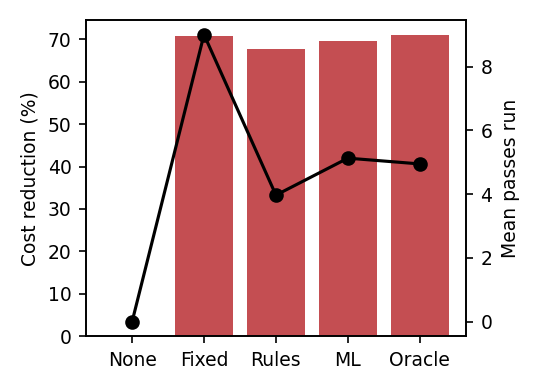
\includegraphics[width=0.6\textwidth]{fig_policies.png}
\caption{Cost reduction (bars) and mean techniques run (line) for each policy.}
\label{fig:policies}
\end{figure}

\subsection{Confidence-Threshold Extension}

\begin{table}[H]
\centering
\caption{Effect of the confidence threshold (Logistic Regression)}
\label{tab:thr}
\begin{tabular}{lcccc}
\toprule
\textbf{Threshold} & \textbf{Fallback rate} & \textbf{Cost red. (\%)} & \textbf{Techniques} & \textbf{Cost-optimal}\\
\midrule
0.0 (none) & 0.0\% & 69.61 & 5.13 & 0.760\\
0.4 & 24.2\% & 70.01 & 6.15 & 0.825\\
0.5 & 50.7\% & 70.42 & 7.15 & 0.893\\
0.6 & 73.9\% & 70.69 & 8.02 & 0.938\\
0.8 & 97.2\% & 70.86 & 8.87 & 0.961\\
\bottomrule
\end{tabular}
\end{table}

\begin{figure}[H]
\centering
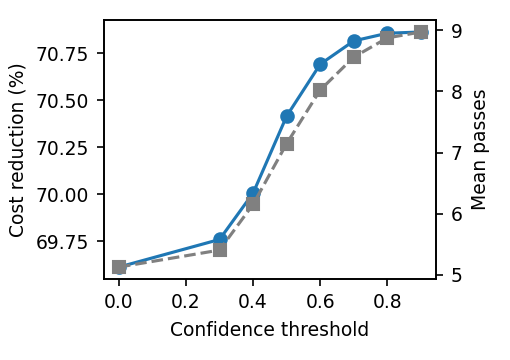
\includegraphics[width=0.55\textwidth]{fig_threshold.png}
\caption{Cost reduction and mean techniques versus confidence threshold.}
\label{fig:threshold}
\end{figure}

\subsection{Confusion Matrix and Feature Importance}

\begin{figure}[H]
\centering
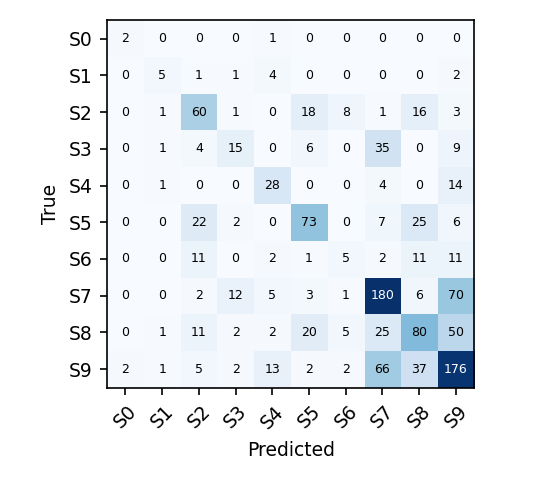
\includegraphics[width=0.55\textwidth]{fig_confusion.png}
\caption{Confusion matrix of the best model on the test set.}
\label{fig:confusion}
\end{figure}

\begin{figure}[H]
\centering
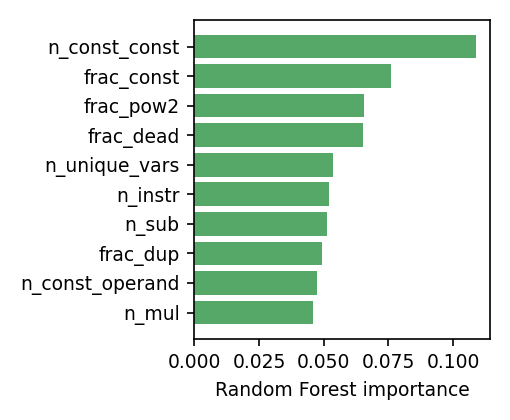
\includegraphics[width=0.55\textwidth]{fig_importance.png}
\caption{Top-10 Random Forest feature importances.}
\label{fig:importance}
\end{figure}

The most important features were the number of constant-only operations
(0.109), the fraction of constant operations (0.076), the fraction of
power-of-two operations (0.066) and the fraction of dead instructions (0.065).

\subsection{Robustness on Longer Programs}

Models trained on programs of 8--40 instructions were tested on 1{,}200 programs
of 45--90 instructions. Accuracy was 0.601, macro F1 was 0.277, cost reduction
was 80.84\% (fixed sequence: 81.24\%), mean techniques run was 7.04 (fixed:
9.0) and the cost-optimal rate was 0.875.

\subsection{Worked Example}

Source input to the front end:

\begin{verbatim}
x = a*8 + b*1
y = a*8 + 0
z = 3*4 + x
w = y + z
v = w * 2
out = v - 0
\end{verbatim}

The front end produces 16 TAC instructions (cost 26). The classifier predicted
sequence S7 (ALG, CSE, CP, DCE) with confidence 0.55, giving 7 instructions
(cost 7), verified equivalent to the original:

\begin{verbatim}
_t1 = a << 3
_t3 = _t1 + b
_t6 = 3 << 2
_t7 = _t6 + _t3
_t8 = _t1 + _t7
_t9 = _t8 + _t8
out = _t9
\end{verbatim}

Note that \verb|3 << 2| remains unfolded because S7 does not include constant
folding; the sequence S8 would have folded it. This illustrates a case where
the model's choice is not the best possible.

\subsection{Discussion}

The main result is that the learned selector keeps most of the benefit of the fixed pipeline while doing less work. Logistic Regression reduced total cost by 69.61\%, compared with 70.86\% for the fixed full sequence and 70.95\% for the oracle, while running 5.13 techniques per program on average instead of 9. This is a saving of about 43\% in compile effort for a loss of about 1.25 percentage points in cost reduction.

The learned selector also outperformed the hand-written rules, which reached 67.74\% cost reduction and chose a cost-optimal sequence for only 58.3\% of programs, against 76.0\% for Logistic Regression. The rules run fewer techniques (3.97) but miss improvements.

The fixed sequence is not a weak baseline. It reached the minimum achievable cost for 96.3\% of programs, so its weakness is wasted effort and not poor code. The learned selector should therefore be understood as an effort-saving method and not as a way of producing better code than the full pipeline. The majority-class baseline predicts the full sequence for every program, because that is the most common label, so its results are identical to those of the fixed sequence.

Exact-sequence accuracy is only 52.0\% for the best model. This is partly because several sequences often give the same cost, so predicting a sequence different from the label does not always make the code worse, and partly because some classes are rare (for example, S0 has only 13 examples). The cost reduction and the cost-optimal rate are therefore more meaningful measures than accuracy here. Logistic Regression and Random Forest performed similarly, Gradient Boosting varied strongly between cross-validation folds (standard deviation 0.113), and the Decision Tree was the weakest.

The confidence threshold gives a controllable trade-off. With no threshold the selector runs 5.13 techniques per program. At a threshold of 0.5, about half of the programs fall back to the full sequence, the cost-optimal rate rises to 0.893 and the mean number of techniques rises to 7.15. At very high thresholds the policy becomes the fixed pipeline.

On longer programs (45--90 instructions) the accuracy was 0.601 but the macro F1 was only 0.277. The cost reduction of 80.84\% remained close to the fixed sequence's 81.24\% while running 7.04 techniques instead of 9. A possible reason is that the count-based features are not normalised for program length and that long programs mostly need the full sequence; this was not tested separately.

The most important features were the number of constant-only operations, the fraction of constant operations, the fraction of power-of-two operations and the fraction of dead instructions. This is sensible, because these features directly indicate whether constant folding, strength reduction and dead-code elimination will help.

\todo{Look at the confusion matrix figure and add one or two sentences naming the classes that are confused most often.}

\subsection{Limitations}

The results have several limitations. First, all programs are synthetic and were produced by our own generator, so the generator's settings shape the results and the findings may not transfer to real software. Second, the programs are straight-line code without loops or branches. Third, the cost model is a simplified latency model and not a measurement of real execution time. Fourth, only five techniques were used, whereas real compilers have many more. Fifth, some classes are rare and the experiments used a single random seed. Finally, semantic equivalence was checked by random testing, which is not a formal proof of correctness.

\newpage

% ============================================================
% CONCLUSION
% ============================================================
\section{Conclusion and Future Work}

\subsection{Conclusion}

This report presented a machine learning framework that selects optimization techniques for three-address code. A classifier uses 22 static features to choose one of ten technique sequences, and the chosen sequence is applied to produce optimized code that is checked for equivalence with the original program.

On 1{,}200 held-out programs, Logistic Regression reduced program cost by 69.6\%, close to the 70.9\% of the fixed full sequence, while running 5.1 techniques instead of 9 on average. It performed better than hand-written rules, and a confidence threshold allows compile effort and code quality to be traded off. The study shows that compile effort can be saved with a small loss in code quality. However, the experiments used only synthetic straight-line programs, so the conclusion should be confirmed on real code.

\subsection{Future Work}

Future work includes evaluating the approach on real code and on real LLVM IR, for example through CompilerGym. An iterative version could predict one technique at a time and re-examine the program after each step, so that any order is possible. The framework could be extended with loops and branches, more optimization techniques, and measured execution time instead of a cost model. Normalising the features by program length and using stronger equivalence checking are further improvements.

\newpage

% ============================================================
% REFERENCES
% ============================================================
% VERIFY every entry (authors, title, venue, year) before submitting.
\begin{thebibliography}{99}

\bibitem{aho2006}
A. V. Aho, M. S. Lam, R. Sethi, and J. D. Ullman,
\textit{Compilers: Principles, Techniques, and Tools},
2nd ed., Pearson, 2006.

\bibitem{cooper2007}
K. D. Cooper and L. Torczon,
\textit{Engineering a Compiler},
2nd ed., Morgan Kaufmann, 2011.

\bibitem{muchnick1997}
S. S. Muchnick,
\textit{Advanced Compiler Design and Implementation},
Morgan Kaufmann, 1997.

\bibitem{cummins2021}
C. Cummins et al.,
``CompilerGym: Robust, performant compiler optimization environments for AI
research,'' arXiv:2109.08267, 2021. % VERIFY authors and venue

\bibitem{liang2023}
H. Liang et al.,
``Learning compiler pass orders using coreset and normalized value
prediction,'' in \textit{Proc. International Conference on Machine Learning
(ICML)}, PMLR vol.\ 202, 2023. % VERIFY authors; also arXiv:2301.05104

\bibitem{pedregosa2011}
F. Pedregosa et al.,
``Scikit-learn: Machine learning in Python,''
\textit{Journal of Machine Learning Research}, vol.\ 12, pp.\ 2825--2830, 2011.
% VERIFY

% TODO: add AutoPhase, MiCOMP and any other papers you have actually read.

\end{thebibliography}

\end{document}
